\documentclass[../main.tex]{subfiles}

\begin{document}

\section{Esfuerzos sísmicos}

\subsection{Ejercicio 1: método estático}

%\href{https://youtu.be/6VVqDEFBOIk}{Clase 1 (20210420)}

\begin{figure}[h]
  \centering
  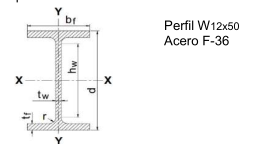
\includegraphics[width=0.8\textwidth]{./images/20210420/ej1}
  \caption{Consigna}
  \label{fig:ej1}
\end{figure}

\begin{figure}[h]
  \centering
  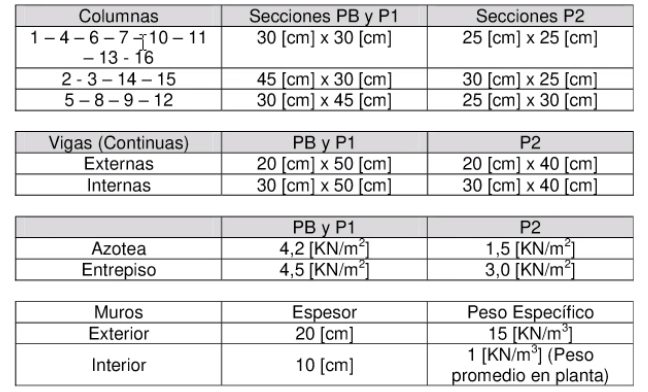
\includegraphics[width=0.8\textwidth]{./images/20210420/ej1_1}
\end{figure}

Las rigideces de piso son $K_{p_2}=\SI{204}{kN / cm}$, $K_{p_1}=\SI{325}{kN /cm}$
 y $K_{pb}=\SI{302}{kN / cm}$

\subsubsection{Determinación de datos básicos}

Del Capítulo 2 del reglamento encontramos:

\begin{itemize}
  \item Zona 4.
  \item Tipo de suelo \textbf{$S_c$}.
  \item Grupo B. $\gamma_r = 1$
  \item Factor de ocurriencia: $f_1=0$ para azotea y  $f_1=0.25$ para oficina.
\end{itemize}

Además, verificamos que estando en una estructura tipo B y estando en una Zona 4,
no superamos una altura de $\SI{45}{m}$. 


\subsubsection{Deterimnación de carga gravitatorio de piso $W_k$}

Según Art. 3.6. Ejemplo para 2º Piso:

\begin{align*}
  \text{Losas} \hspace{0.25cm} &\xrightarrow{\hspace*{0.5cm}} \hspace{0.1cm} 
    \SI{18}{m} * \SI{18}{m} * \SI{4.2}{kN /m^2} = \SI{1360.8}{kN} \\[5pt] 
  \text{Vigas} \hspace{0.25cm} &\xrightarrow{\hspace*{0.5cm}} \hspace{0.1cm} (4 * 
    \SI{0.20}{m} * \SI{0.4}{m} * \SI{18}{m} + \SI{0.3}{m}*\SI{0.4}{m}*\SI{18}{m}) * 25 
    = \SI{360}{kN} \\[5pt]
  \text{Columnas} \hspace{0.25cm} &\xrightarrow{\hspace*{0.5cm}} \hspace{0.1cm}
    8*((\SI{0.25}{m}*\SI{0.25}{m}+\SI{30}{m}*\SI{25}{m})*\SI{1.6}{m})*\SI{25}{kN /m^3} 
    = \SI{44}{kN} \\[5pt]
  \text{Muros} \hspace{0.25cm} &\xrightarrow{\hspace*{0.5cm}} \hspace{0.1cm}
    4*(\SI{2}{m}*\SI{0.2}{m}*\SI{18}{m}))*\SI{15}{kN /m^2} + 4 * (\SI{1.6}{m} * 
    \SI{0.2}{m} * \SI{18}{m})*\SI{15}{kN /m^3} = \SI{777.6}{kN}
.\end{align*}

El total de esto nos dará $G_3=\SI{2542.4}{kN}$. Realizando lo mismo para los otros
pisos tenemos $G_2 = \SI{3067}{kN}$ y $G_1 = \SI{3171.5}{kN}$.

Agregamos a esto el factor de ocurrencia, y lo multiplicamos por una carga de
$\SI{3}{kN / m^2}$ por el área del piso. Entonces:

\begin{align*}
  W_3 &= \SI{2542}{kN} \\[5pt]
  W_2 &= \SI{3310}{kN} \\[5pt]
  W_1 &= \SI{3415}{kN}
.\end{align*}

\subsubsection{Cálculo de fuerza fundamental}

Primero, sabemos que la fuerza será:

\begin{align*}
  F_i = \frac{W_i*h_i}{\Sigma W_i * h_i}
.\end{align*}

Luego, podemos aplicar una matriz como la que sigue:

\begin{align*}
\begin{bmatrix} 
  K_{pb}+K_{p1} & -K_{p1}       & 0 \\
  -K_{p1}       & K_{p1}+K_{p2} & -K_{p2} \\
  0             & K_{p2}        & K_{p2} 
\end{bmatrix} 
\times \begin{bmatrix} U_1 \\ U_2 \\ U_3 \end{bmatrix} 
= \begin{bmatrix} F_1 \\ F_2 \\ F_3 \end{bmatrix} 
\tag{Matriz deformaciones}\label{matriz-def}\end{align*}

Todo esto es posible automatizarlo con la siguiente tabla:

\begin{figure}[ht]
  \centering
  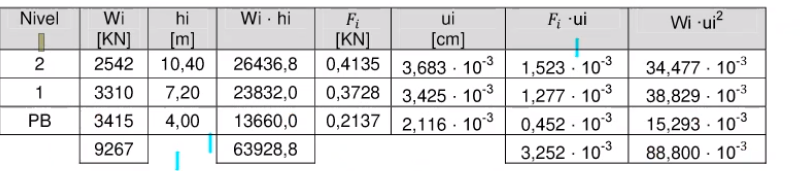
\includegraphics[width=0.8\textwidth]{./images/20210420/tabla_calc}
  \caption{Tabla de calculo}
  \label{fig:tabla_calc}
\end{figure}

Y aplicando \cref{matriz-def} podemos sacar las deformaciones, y por último también
podemos encontrar el periodo de la siguiente forma:

\begin{align*}
  T &= 2 * \pi * \sqrt{\frac{\sigma W_i * u_i^2}{g*\sigma F_i*u_i}}  \\[5pt]
  T &= 2*\pi \sqrt{\frac{88.8*10^{-3}}{\SI{981}{cm / s^2}*3.252*10^{-3}}} = \SI{1.05}{s}
.\end{align*}

Luego debemos obtener el \textbf{período fundamental aproximado},
denominado $T_a$, y compararlo y adoptar el menor entre los dos valores de 
períodos obtenidos.

\begin{align*}
  T_a = C_r * H^x = 0.0466 * 10.4^{0.9} = \SI{0.38}{s} 
.\end{align*}

Luego, verificamos la condición del Art. 6.2.3. que dice que el valor de período
a utilizar debe cumplir con $T \leq C_u * T_a$. En nuestro caso, $C_i = 1.4 $, 
en función de  $a_s = 0.35$ que sale de la Tabla 3.1 del CIRSOC 103. Esto nos indica
que el valor del período a adoptar será:

\begin{align*}
  T = T_a * 1.4 = 0.38 * 1.4 = \SI{0.53}{s}
.\end{align*}

 Vemos que tenemos que tenemos que entonces adoptar el valor de $T = \SI{0.53}{s}$.

% COMPLETAR

\end{document}
